% ========================================
\section{Numerical experiments}\label{sec:Num-Exp}
% ========================================
%
We present numerical results for both Monte Carlo and multi-fidelity Monte Carlo sampling methods to estimate the expectation $\mathbb{E}(u)$. Following \cite{FaHe:2017}, the computational framework is built upon an ITER reactor geometry featuring twelve magnetic coils, with the \textit{reference currents} $\boldsymbol{I}$ specified as
%
\begin{equation}\label{eq:CentralCurrentValue}
{\renewcommand{\arraycolsep}{2pt}
\begin{array}{llll}
I_1 = -1.4 \times 10^{6} A, \quad & I_2 = -9.5 \times 10^{6} A, \quad & I_3 = -2.0388 \times 10^{7} A, \quad & I_4 = -2.0388 \times 10^{7} A, \\
I_5 = -9 \times 10^{6} A, \quad & I_6 = 3.564 \times 10^{6} A, \quad & I_7 = 5.469 \times 10^{6} A, \quad & I_8 = -2.266 \times 10^{6} A, \\
I_9 = -6.426 \times 10^{6} A, \quad & I_{10} = -4.82 \times 10^{6} A, \quad & I_{11} = -7.504 \times 10^{6} A, \quad & I_{12} = 1.724 \times 10^{7} A. 
\end{array}
}
\end{equation}
%
The profiles for $p$ and $g$ on the right-hand side of \eqref{eq:FreeBoundary} follow the form given in \eqref{eq:source}, using the following \textit{reference parameter} values
%
\begin{equation}\label{eq:CentralParameterValue}
r_0=6.2m,\,\,\beta=0.5978, \,\, \alpha_1 = 2, \,\,  \alpha_2=1.395, \,\, j_0=1.3655 \times 10^6 A/m^2,\,\,  \mu_0=1.2566\times 10^{-6} N/A^2.
\end{equation}
%
To evaluate the sensitivity of the solution to \eqref{eq:FreeBoundary} under uncertainty, we conduct two experiments, each introducing a specific source of variability. In the first experiment, uncertainties are introduced in the coil currents, modeled as uniformly distributed perturbations of $\tau = 2\%$ around the reference currents in \eqref{eq:CentralCurrentValue}, while the profile parameters are held fixed at their reference values, isolating the impact of current variability on the solution. The reactor geometry and coil arrangement adhere to the descriptions provided in \cite{Amoskov:2009}.  A family of nested spatial meshes $\{\mathcal{T}_k\}$ is generated by refining and coarsening the reference ITER geometry, yielding six distinct spatial discretizations, with the number of spatial grid nodes $\{M_\ell,\}_{0\le \ell \le 5}$  satisfying
%
\begin{equation}
\label{eq:MeshGrowth}
M_\ell = s M_{\ell-1} \qquad \text{ for } s>1.
\end{equation}
%
The number of the available spatial grid nodes are shown in the first row of Table \ref{Tab:Dof}.
% \sout{In the second experiment, uncertainties are introduced in the profile parameters, modeled as uniformly distributed perturbations of $\tau = 1\%$ around the reference values in \eqref{eq:CentralParameterValue}, with the coil currents kept constant.}

The splitting ratio $\theta$ is set to 0.5 to reflect a balance between discretization and statistical errors. The tolerances for the normalized mean square error are selected to slightly exceed the discretization error on the finest available mesh $(\ell=5)$, with specific values being $\epsilon=2\times 10^{-4}, 4\times 10^{-4}, 6\times 10^{-4}, 8\times 10^{-4}, 1\times 10^{-3}, 2\times 10^{-3}, 4\times 10^{-3}, 8\times 10^{-3}$. For each tolerance, the corresponding spatial grid level required to satisfy the discretization error thresholds is determined using the relation described in \eqref{eq:SLSGC_MLS_SpatialGridsNo}, resulting in levels $L = 5, 4, 4, 4, 4, 3, 3, 2, 2$. The high-fidelity model for each tolerance corresponds to the finite element solution of \eqref{eq:FreeBoundary} on the spatial grid level $L$. For each high-fidelity model defined on the spatial grid level $L$, candidate low-fidelity surrogates are constructed using the sparse grid stochastic collocation approach outlined in Section \ref{sec:SC}. These surrogates are generated using sparse grid nodes \eqref{eq:NestedColPts} of level $q=1$, and are defined over a sequence of spatial meshes with grid levels ranging from $0$ to $L-1$, where $L$ denotes the spatial grid level of the corresponding high-fidelity model. 

To perform MFMC sampling, accurately estimating the statistical parameters, such as the mean and correlation coefficients that characterize the correlation between high- and low-fidelity models is of critical importance. The calculation of correlation coefficients requires the knowledge of variance and covariance. To achieve robust and numerically stable updates for these sample statistics, Welford's algorithm \cite{Welford:1962} is used for both high- and low-fidelity models. The initialization of the proxies for the mean and variance of the high- and low-fidelity models is set to $m_w^{(1)}=0$, $v_w^{(1)}=0$, $\widehat m_w^{(1)}=0$, and $\widehat v_w^{(1)}=0$, respectively.  For the high-fidelity model  $\widehat u_{h,1}=u_h$, the proxies for the sample mean and variance are updated iteratively as new samples are incorporated through the recurrence relations
%
\[
m_w^{(i)} = m_w^{(i-1)} + \frac{u_h\left(\boldsymbol{\omega}^{(i)}\right)-m_w^{(i-1)}}{i},\qquad v_w^{(i)} = v_w^{(i-1)} + \left\langle u_h\left(\boldsymbol{\omega}^{(i)}\right)-m_w^{(i-1)}, \;\;u_h\left(\boldsymbol{\omega}^{(i)}\right)-m_w^{(i)}\right\rangle,
\]
%
Similarly, for the low-fidelity model $\widehat u_{h,k}$, the proxies are updated using analogous recurrence relations
%
\[
\widehat m_w^{(i)} = \widehat m_w^{(i-1)} + \frac{\widehat u_{h,k}\left(\boldsymbol{\omega}^{(i)}\right) - \widehat m_w^{(i-1)}}{i},\qquad \widehat v_w^{(i)} = \widehat v_w^{(i-1)} + \left\langle \widehat u_{h,k}\left(\boldsymbol{\omega}^{(i)}\right)-\widehat m_w^{(i-1)},\;\; \widehat u_{h,k}\left(\boldsymbol{\omega}^{(i)}\right)-\widehat m_w^{(i)}\right\rangle,
\]
%
The correlation between the high- and low-fidelity models is quantified through the covariance, for which the proxy is initialized as $r_w^{(1)}=0$. The iterative update for the covariance is performed using the relation
%
\[
r_w^{(i)} = r_w^{(i-1)} + \left \langle u_{h}\left(\boldsymbol{\omega}^{(i)}\right)-m_{w}^{(i-1)},\;\;\widehat u_{h,k}\left(\boldsymbol{\omega}^{(i)}\right)-\widehat m_{w}^{(i)}\right\rangle,
\]
%
These iterative updates ensure that the statistical parameters are dynamically adjusted without requiring the storage of all previous samples, thus maintaining computational efficiency. Using these updated proxies, the sample standard deviations of the high- and low-fidelity models are calculated as $\sigma^{(i)} = \sqrt{v_w^{(i)}/(i-1)}$ and $\widehat \sigma^{(i)} = \sqrt{\widehat v_w^{(i)}/(i-1)}$ respectively. The sample covariance between the high-fidelity model and each low-fidelity model is determined as $\text{Cov}^{(i)} = r_w^{(i)}/(i-1)$.

Experiments were performed using MATLAB R2024a on the batch-scheduled HPC/HTC cluster NOTSx, part of the Rice Big Research Data cloud infrastructure. The system consists of 298 dual-socket compute blades housed on HPE s6500, HPE Apollo 2000, and Dell PowerEdge C6400 chassis. All nodes are interconnected via a high-speed network with 10 or 25 Gigabit Ethernet.


% =============================
\subsection{Surrogate construction and parameter estimation (offline) costs}
% =============================
We first estimate the statistical parameters using high fidelity and candidate low-fidelity surrogate models for each given tolerance $\epsilon$. To avoid introducing statistical dependence between parameter estimates, each pairwise parameter (e.g., correlation coefficient $\rho_{1,k}$ between high-fidelity and the $k$-th low-fidelity model) is estimated using mutually independent sample sets. Specifically, for $K$ low-fidelity models where estimating each  $\rho_{1,k}$ requires $N$ independent high-fidelity samples, the total number of high-fidelity evaluations becomes $KN$. Table \ref{Tab:MFMC_parameters} presents these estimates for predetermined thresholds $\epsilon$, including standard deviations, covariance and correlation coefficients between the high-fidelity model and each candidate low-fidelity model. We implement Welford's method to iteratively update sample statistics while adaptively increasing sample sizes until convergence criteria are met, terminating when relative differences between successive updates fall below $10^{-4}$. These parameters are then used in Algorithm \ref{algo:MFMC_Algo_model_selection} to select the optimal low-fidelity models for MFMC. 


% The selection of low-fidelity models, performed using Algorithm \ref{algo:MFMC_Algo_model_selection}, relies on the accurate computation of these statistical quantities, which directly impact the efficiency of the MFMC framework, the required sample size, and the overall computational cost. Errors in these estimates can lead to suboptimal model selection, excessive sampling that increases computational overhead, or insufficient sampling that compromises accuracy.


%
\begin{table}[ht]
\centering
\scalebox{0.8}{
\begin{tabular}{|c|c|c|c|c|c|c|c|c|c|c|c|c|c|c|c|c|c|c|}
\cline{1-8}	
\multirow{2}{*}{$\epsilon$}&\multicolumn{1}{|c|}{$\ell$} &0&1&2&3&4&5\\
\cline{2-8}	
&\multicolumn{1}{|c|}{$M_\ell$} &$2685$ &$8019$ &$30449$ &$120697$ &$484080$ &$1934365$\\
\hline
\multirow{4}{*}{$6\times 10^{-3}\;\;\sim \;\;8\times 10^{-3}$} &\multicolumn{1}{|c|}{Candidate model $k$} &$\widehat u_{h,3}$&$\widehat u_{h,2}$&$\widehat u_{h,1}$&\multirow{4}{*}{}&\multirow{4}{*}{}&\multirow{4}{*}{}\\
\cline{2-5}		
&\multicolumn{1}{|c|}{$\sigma_{k}$}&9.5720e-03   &1.1549e-02   &1.0939e-02&&&\\
\cline{2-5}	
&\multicolumn{1}{|c|}{$\text{Cov}\left(\widehat u_{h,1},\widehat u_{h,k}\right)$}&1.0286e-04&1.2604e-04&-&&&\\
\cline{2-5}
&\multicolumn{1}{|c|}{$\rho_{1,k}$}&9.8238e-01&9.9762e-01&-&&&\\
\hline
\hline
\multirow{4}{*}{$2\times 10^{-3}\;\;\sim \;\;4\times 10^{-3}$} &\multicolumn{1}{|c|}{Candidate model $k$} &$\widehat u_{h,4}$&$\widehat u_{h,3}$&$\widehat u_{h,2}$&$\widehat u_{h,1}$&\multirow{4}{*}{}&\multirow{4}{*}{}\\
\cline{2-6}	
 % &\multicolumn{1}{|c|}{$\sigma_{1}$}&\multicolumn{3}{c|}{}&1.1742e-04&&\\
 % \cline{2-6}	
&\multicolumn{1}{|c|}{$\sigma_{k}$}&9.5720e-03   &1.1549e-02   &1.1001e-02   &1.0836e-02 &&\\
\cline{2-6}	
&\multicolumn{1}{|c|}{$\text{Cov}\left(\widehat u_{h,1},\widehat u_{h,k}\right)$} &1.0206e-04 &1.2480e-04 &1.1911e-04 &- &&\\
\cline{2-6}	
&\multicolumn{1}{|c|}{$\rho_{1,k}$}&9.8394e-01&9.9720e-01 &9.9919e-01&-&&\\
\hline
\hline
\multirow{4}{*}{$4\times 10^{-4}\;\;\sim \;\;1\times 10^{-3}$} &\multicolumn{1}{|c|}{Candidate model $k$} &$\widehat u_{h,5}$&$\widehat u_{h,4}$&$\widehat u_{h,3}$&$\widehat u_{h,2}$&$\widehat u_{h,1}$&\multirow{4}{*}{}\\
 \cline{2-7}	
&\multicolumn{1}{|c|}{$\sigma_{k}$}&9.5720e-03   &1.1549e-02   &1.1001e-02   &1.0838e-02   &1.0840e-02  &\\
\cline{2-7}	
&\multicolumn{1}{|c|}{$\text{Cov}\left(\widehat u_{h,1},\widehat u_{h,k}\right)$}&1.0209e-04 &1.2485e-04 &1.1916e-04 &1.1745e-04 &- &\\
\cline{2-7}	
&\multicolumn{1}{|c|}{$\rho_{1,k}$}&9.8392e-01 &9.9727e-01 &9.9925e-01 &9.9977e-01 &- &\\
\hline
\hline
\multirow{4}{*}{$2\times 10^{-4}$} &\multicolumn{1}{|c|}{Candidate model $k$} &$\widehat u_{h,6}$&$\widehat u_{h,5}$&$\widehat u_{h,4}$&$\widehat u_{h,3}$&$\widehat u_{h,2}$&$\widehat u_{h,1}$\\
\cline{2-8}
&\multicolumn{1}{|c|}{$\sigma_{k}$}&9.5720e-03   &1.1549e-02   &1.1001e-02   &1.0838e-02   &1.0812e-02  &1.0840e-02\\
\cline{2-8}	
&\multicolumn{1}{|c|}{$\text{Cov}\left(\widehat u_{h,1},\widehat u_{h,k}\right)$}&1.0209e-04&1.2485e-04&1.1916e-04&1.1745e-04&1.1717e-04&-\\
\cline{2-8}	
&\multicolumn{1}{|c|}{$\rho_{1,k}$}&9.8390e-01   &9.9728e-01   &9.9925e-01   &9.9977e-01   &9.9976e-01   &-\\
\hline
\end{tabular}}
\caption{Estimated statistical parameters for various predetermined tolerances $\epsilon$ in terms of nMSE. The high-fidelity model $\widehat u_{h,1}$ represents the finite element solution to the free boundary problem on a spatial grid of level $L$, ensuring the discretization error meets accuracy requirements. Candidate low-fidelity models $\widehat u_{h,k}$ for $k \geq 2$ are generated using 25 sparse grid nodes (with level $q=1$) on spatial grids from levels 0 to $L-1$. All parameters are estimated using Welford's dynamic sampling algorithm with a stopping criterion requiring a relative error of $10^{-4}$ for all parameters.}
\label{Tab:MFMC_parameters}
\end{table}
%


To evaluate the computational efficiency of the MFMC method, we next quantify the per-sample evaluation costs for both the high-fidelity model $(W_\ell)$ and its corresponding low-fidelity surrogates $(W_\ell^e)$ across mesh levels ranging from $0$ to $5$. These costs, summarized in Table \ref{Tab:Dof}, reflect the computational workload required for a single evaluation at each fidelity level. The costs are generated with the same experiment used for estimating statistical parameters at the tolerance threshold $\epsilon=2\times 10^{-4}$, as shown in the final block of Table \ref{Tab:MFMC_parameters}. Let $L$ be the finest spatial grid level required for the high-fidelity model to satisfy the discretization error, for a given tolerance $\epsilon$, then the cost per sample for the MFMC is related to the cost in Table \ref{Tab:Dof} as $C_1=W_{L}$ and $C_k=W_{L-k+1}^e$.

%
\begin{table}[ht]
\centering
\scalebox{0.8}{
\begin{tabular}{c|c|c|c|c|c|c|c|c|c|c|c|c|c|c|c|c|c|c|}
\cline{1-7}	
\multicolumn{1}{|c|}{$\ell$} &0&1&2&3&4&5\\
\hline
\multicolumn{1}{|c|}{$M_\ell$} &$2685$ &$8019$ &$30449$ &$120697$ &$484080$ &$1934365$\\
% \hline
% \multicolumn{1}{|c|}{Model $k$} &$f_1$&$f_2$&$f_3$&$f_4$&$f_5$&$f_6$\\
\hline
\multicolumn{1}{|c|}{$W_\ell$ direct solve}&4.88e-02 &1.49e-01 &6.33e-01 &3.23e+00 &1.55e+01 &7.30e+01\\
\hline
\multicolumn{1}{|c|}{$W_\ell^e$ surrog evaluation}&2.68e-04   &5.06e-04   &1.40e-03   &7.03e-03   &2.17e-02   &9.71e-02\\
\hline
% \multicolumn{1}{|c|}{$C_\ell$ surrog evaluation( nodes)-source term}&\\
% \hline
\end{tabular}}
\caption{The number of spatial grid points $M_\ell$, cost per sample for both direct computation $W_\ell$ and surrogate evaluation $W_\ell^e$ at an increasing spatial grid level $\ell = 0$ to 5.}
% and surrogate evaluation with level $q=1$ sparse grid nodes ($P=$)  in the source term.}
\label{Tab:Dof}
\end{table}
%

%
\begin{figure}[ht!]\centering
\begin{tabular}{cc}
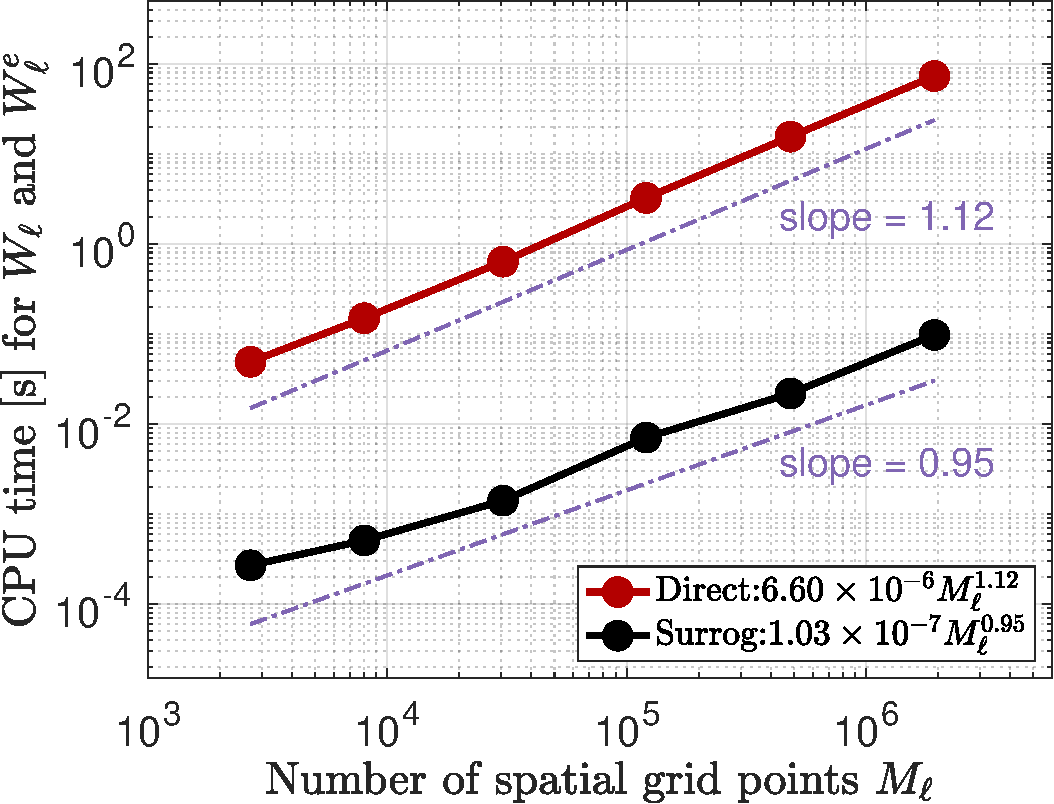
\includegraphics[width=0.46\linewidth]{./figures/CostPerSample_Ml.pdf}
% \includegraphics[width=0.46\linewidth]{./Figures/Surrog_Construct_Cost.pdf}
\end{tabular}
\caption{Left:  Mean CPU times to compute 500 realizations of solutions for direct computations vs.\ an increasing number of spatial grid points $M_\ell$. Right:  Offline costs of construction of ...}
\label{fig:CostEstimatePlot}
\end{figure}
%


 Table \ref{Tab:Offline_cost} quantifies the total offline computational cost (measured in CPU time) incurred during the preparatory phase of the MFMC framework.  This cost comprises two primary components: the computational expense associated with constructing low-fidelity surrogate models across spatial mesh levels  $\ell = 0, \ldots, L-1$, where $L$ denotes the finest spatial grid resolution satisfying the prescribed discretization error tolerance $\theta\epsilon^2$, and the cost of estimating statistical parameters (e.g., variances $\sigma_k^2$, correlation coefficients $\rho_{1,k}$) required for MFMC, as detailed in Table \ref{Tab:MFMC_parameters}. While the offline preparation incurs non-negligible computational expenses, these costs are justified by the substantial savings achieved during large-scale online sampling, particularly in applications requiring thousands of high-fidelity model evaluations. As a one-time expense, the precomputed surrogates and statistical parameters are reused throughout the online phase, amortizing the initial overhead across all subsequent multi-fidelity Monte Carlo realizations.

%
\begin{table}[ht]
\centering
\scalebox{0.8}{
\begin{tabular}{c|c|c|c|c|c|c|c|c|c|c|c|c|c|c|c|c|c|c|}
\hline
\multicolumn{1}{|c|}{$\epsilon$} &$8\times 10^{-3}$&$6\times 10^{-3}$&$4\times 10^{-3}$&$2\times 10^{-3}$&$10^{-3}$&$8\times 10^{-4}$&$6\times 10^{-4}$&$4\times 10^{-4}$&$2\times 10^{-4}$\\
\hline
\multicolumn{1}{|c|}{Build surrogate }&2.11e+01&2.11e+01&1.08e+02&1.08e+02&5.53e+02&5.53e+02&5.53e+02&5.53e+02&2.39e+03\\
\hline
\multicolumn{1}{|c|}{Estimate parameters}&2.80e+03&2.80e+03&6.08e+03&6.08e+03&1.68e+04&1.68e+04&1.68e+04&1.68e+04&6.9423e+04\\
% &2.02e+00&7.90e+00&3.10e+01&1.52e+02&8.12e+02&3.56e+03\\
\hline
\end{tabular}
}
\caption{The offline cost. The second row--CPU time to construct surrogate $\widehat u_{h,k}$ with sparse grid level $q=1$ with respect to decreasing tolerance. The third row corresponds to the total time to estimate the parameters with 500 samples, this cost includes evaluation of surrogate and direct computation, interpolation to solution to the common fine mesh, and use Welford's algorithm to compute the sample statistics.}
\label{Tab:Offline_cost}
\end{table}
%



% %
% \begin{table}[ht]
% \centering
% \scalebox{0.8}{
% \begin{tabular}{c|c|c|c|c|c|c|c|c|c|c|c|c|c|c|c|c|c|c|}
% \cline{1-7}	
% \multicolumn{1}{|c|}{$\ell$} &0&1&2&3&4&5\\
% \hline
% \multicolumn{1}{|c|}{$M_\ell$} &$2685$ &$8019$ &$30449$ &$120697$ &$484080$ &$1934365$\\
% \hline
% \multicolumn{1}{|c|}{Model $k$} &$\widehat u_{h,5}$&$\widehat u_{h,4}$&$\widehat u_{h,3}$&$\widehat u_{h,2}$&&\\
% \hline
% \multicolumn{1}{|c|}{$\rho_{1,k}$ (24 nodes), ref l=3}&0.9802&0.9958 &0.9976&0.9984&&\\
% \hline
% \multicolumn{1}{|c|}{$\sigma_{k}$}&9.3826e-05 &1.374e-04 &1.2405e-04 &1.2016e-04 &&\\
% \hline
% \multicolumn{1}{|c|}{Covariance} &1.0807e-04 &1.3283e-04 &1.2646e-04 &1.2457e-04 &&\\
% \hline
% \end{tabular}}
% \caption{$\epsilon = 4\times 10^{-3}\;\;\& \;\;2\times 10^{-3}$. High fidelity model: finite element solution on mesh with 120697 grid nodes. $\sigma_1 = 1.2955e-04$. The data are estimated using 500 samples. The selected models are $[\widehat u_{h,2},\widehat u_{h,4},\widehat u_{h,5}]$.}
% % \label{Tab:Dof}
% \end{table}
% %

% %
% \begin{table}[ht]
% \centering
% \scalebox{0.8}{
% \begin{tabular}{c|c|c|c|c|c|c|c|c|c|c|c|c|c|c|c|c|c|c|}
% \cline{1-7}	
% \multicolumn{1}{|c|}{$\ell$} &0&1&2&3&4&5\\
% \hline
% \multicolumn{1}{|c|}{$M_\ell$} &$2685$ &$8019$ &$30449$ &$120697$ &$484080$ &$1934365$\\
% \hline
% \multicolumn{1}{|c|}{Model $k$} &$\widehat u_{h,6}$&$\widehat u_{h,5}$&$\widehat u_{h,4}$&$\widehat u_{h,3}$&$\widehat u_{h,2}$&\\
% \hline
% \multicolumn{1}{|c|}{$\rho_{1,k}$ (24 nodes), ref l=3}&9.0103e-01 &9.2531e-01 &9.2415e-01 &9.2366e-01 &9.2307e-01 &\\
% \hline
% \multicolumn{1}{|c|}{$\sigma_{k}$}&1.1064e-04 &1.3571e-04 &1.2930e-04 &1.2757e-04  &1.2742e-04  &\\
% \hline
% \multicolumn{1}{|c|}{Covariance}&8.9789e-05 &1.2808e-04 &1.1657e-04 &1.1358e-04 &1.1346e-04 &\\
% \hline
% \end{tabular}}
% \caption{$\epsilon = 1\times 10^{-3}\;\;\& \;\;8\times 10^{-4}\;\;\& \;\;6\times 10^{-4}\;\;\& \;\;4\times 10^{-4}$. High fidelity model: finite element solution on mesh with 484080 grid nodes. $\sigma_1 = 1.6794e-04$. The data are estimated using 500 samples.}
% % \label{Tab:Dof}
% \end{table}
% %

% %
% \begin{table}[ht]
% \centering
% \scalebox{0.8}{
% \begin{tabular}{c|c|c|c|c|c|c|c|c|c|c|c|c|c|c|c|c|c|c|}
% \cline{1-7}	
% \multicolumn{1}{|c|}{$\ell$} &0&1&2&3&4&5\\
% \hline
% \multicolumn{1}{|c|}{$M_\ell$} &$2685$ &$8019$ &$30449$ &$120697$ &$484080$ &$1934365$\\
% \hline
% \multicolumn{1}{|c|}{Model $k$} &$\widehat u_{h,7}$&$\widehat u_{h,6}$&$\widehat u_{h,5}$&$\widehat u_{h,4}$&$\widehat u_{h,3}$&$\widehat u_{h,2}$\\
% % \hline
% % \multicolumn{1}{|c|}{$C_k$ direct solve}&1.2029e+02&2.6478e+01&5.3710e+00&1.1269e+00&2.9300e-01&9.6419e-02\\
% % \hline
% % \multicolumn{1}{|c|}{$C_k$ surrog evaluation(24 nodes)}&1.2595e-01&2.9694e-02&9.1085e-03&3.0580e-03&1.1869e-03&2.5127e-04\\
% \hline
% \multicolumn{1}{|c|}{$\rho_{1,k}$ (24 nodes), ref l=3}&1.0095e+00   &1.0092e+00   &1.0095e+00   &1.0090e+00   &1.0091e+00   &9.9033e-01\\
% \hline
% \multicolumn{1}{|c|}{$\sigma_{k}$}&1.2775e-04   &1.2804e-04   &1.2796e-04   &1.3161e-04   &1.4586e-04   &9.7734e-05\\
% \hline
% \multicolumn{1}{|c|}{Covariance}&1.3872e-04   &1.3885e-04   &1.3884e-04   &1.4073e-04   &1.4817e-04   &1.1903e-04\\
% \hline
% \end{tabular}}
% \caption{$\epsilon = 2\times 10^{-4}$. High fidelity model: finite element solution on mesh with 1934365 grid nodes. $\sigma_1 = 1.4782e-04$. The data are estimated using 100 samples. Total time: 1.6676e+04  + 1.5951e+04 +  1.6914e+04 + 1.7699e+04 +  1.7657e+04 + 1.7683e+04}
% % \label{Tab:Dof}
% \end{table}
% % 



% =============================
\subsection{Sampling (online) cost}
% =============================
After the offline procedure, we obtain the necessary parameters and low-fidelity models for estimating the MFMC estimator in the online process. In \eqref{eq:MFMC_estimator_independent}, if the weights $\alpha_k$ are deterministic (theoretically optimal), the estimator is unbiased since $\mathbb{E}(\alpha_k Y_k) = \alpha_k \mathbb{E}(Y_k)$ and $\mathbb{E}(Y_k) = 0$ for $k=2,\ldots, K$. However, if we reuse samples for parameter estimation with those used in the online sampling for $A^{\text{MF}}$, the weights $\alpha_k$ become random variables dependent on the samples and correlated with the correction term $Y_k$. In this case, $\mathbb{E}(\alpha_k Y_k) = \mathbb{E}(\alpha_k Y_k)-\mathbb{E}(\alpha_k)\mathbb{E}(Y_k) = \text{Cov}(\alpha_k,Y_k)\neq 0$ and $\mathbb{E}(A^{\text{MF}})\neq \mathbb{E}(Y_1)$, potentially introducing bias into the estimator. To preserve unbiasedness, samples for parameter estimation must be statistically independent from those used in online sampling. This ensures that $\alpha_k$ and $Y_k$ remain uncorrelated, maintaining $\mathbb{E}(A^{\text{MF}})= \mathbb{E}(Y_1)$.
If reusing offline samples is necessary, the offline sample size should be sufficiently large to ensure that $\alpha_k$ approximates its theoretical value, and the online samples must remain independent of the offline samples to eliminate the correlation between $\alpha_k$ and $Y_k$.






% \JLcolor{According to \cite{PeGuWi:2018}, pages A3174 and A3181–A3182, perturbations in the sample variance and sample correlation coefficients have a small impact on the overall sample size and computational work. However, from my perspective, inaccurate estimation of these statistical parameters can also affect the model selection process. If these statistics are not reliably computed, low-fidelity models with misleading characteristics may be selected or rejected incorrectly, potentially undermining the efficiency and accuracy of the MFMC framework. In particular, models that exhibit inconsistent statistical properties violating the two conditions in Theorem \ref{thm:Sample_size_est} could be included, leading to suboptimal model choices for the low-fidelity approximations and, consequently, affecting the overall performance of the multi-fidelity estimator.}






% =============================
\subsection{Properties of geometric discriptors}
% =============================
As demonstrated in \cite{ElLiSa:2023}, multilevel Monte Carlo (MLMC) implementations face significant challenges when dealing with plasma boundary distortions caused by extrapolation errors during cross-level sample correction aggregation on non-nested, geometry-conforming meshes. These errors arise from mismatches in spatial resolution when coarse-grid corrections are accumulated across multiple levels. This distortion can be mitigated by interpolating the multilevel solutions onto a unified fine grid with level $\ell=5$, effectively reconciling resolution disparities while preserving the geometric fidelity of the plasma boundary. Similarly, in the multi-fidelity Monte Carlo (MFMC) approach, sample corrections for various low-fidelity models are generated using stochastic collocation on the same non-nested, uniform, geometry-conforming coarse grids. To ensures that all corrections are aligned on a consistent spatial resolution for generating the multi-fidelity estimator for the expected plasma field in \eqref{eq:QoI}, it is necessary to project these corrections onto a common fine mesh, enabling accurate and reliable estimation of the quantity of interest. Figure \ref{fig:QoI_plot} shows the contour plot of plasma boundary of the \eqref{eq:QoI} for Monte Carlo, multilevel Monte Carlo and multi-fidelity Monte Carlo samplings. We observe that the plasma boundary resulting from the multi-fidelity Monte Carlo behaves in a similar fashion as that in the benchmark sampled with Monte Carlo.

%=====================================================================================
\noindent \textbf{Plasma boundary.} 
%=====================================================================================






% %
% \begin{table}[ht]
% \centering
% \scalebox{0.8}{
% \begin{tabular}{c|c|c|c|c|c|c|c|c|c|c|c|c|c|c|c|c|c|c|}
% \cline{1-7}	
% \multicolumn{1}{|c|}{Dof} &$1934365$&$484080$&$120697$&$30449$&$8019$&$2685$\\
% \hline
% \multicolumn{1}{|c|}{Model $k$} &$f_1$&$f_2$&$f_3$&$f_4$&$f_5$&$f_6$\\
% % \hline
% % \multicolumn{1}{|c|}{$C_k$ direct solve}&1.2029e+02&2.6478e+01&5.3710e+00&1.1269e+00&2.9300e-01&9.6419e-02\\
% % \hline
% % \multicolumn{1}{|c|}{$C_k$ surrog evaluation(24 nodes)}&1.2595e-01&2.9694e-02&9.1085e-03&3.0580e-03&1.1869e-03&2.5127e-04\\
% \hline
% \multicolumn{1}{|c|}{$\rho_{1,k}$ (24 nodes), ref l=3}&&&&0.9678&0.9670&0.9488\\
% \hline
% \multicolumn{1}{|c|}{$\sigma_{k}$}&&&&1.1696e-04&1.2929e-04&8.8977e-05\\
% \hline
% \multicolumn{1}{|c|}{Covariance}&&&&1.3065e-04&1.3726e-04&1.1172e-04\\
% \hline
% \end{tabular}}
% \caption{High fidelity model: finite element solution on mesh with 30449 grid nodes. $\sigma_1 = 1.5582e-04$. The data are estimated using 500 samples.}
% % \label{Tab:Dof}
% \end{table}
% %









   

   


\begin{figure}[ht!]\centering
\begin{tabular}{ccc}
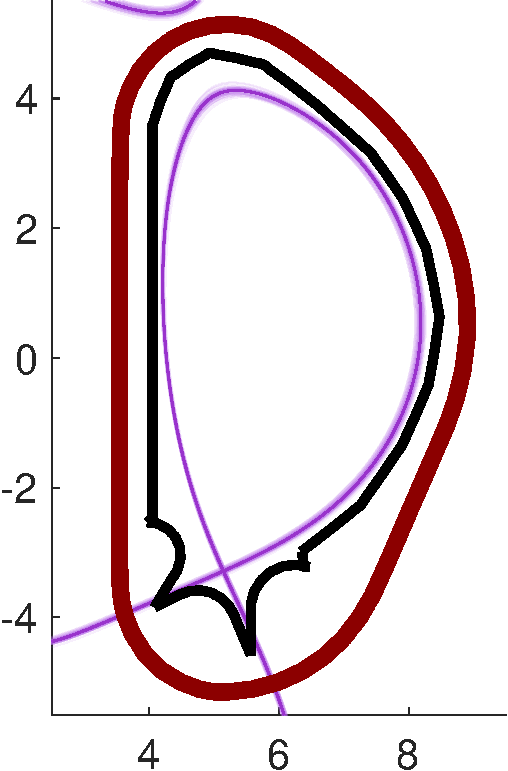
\includegraphics[width=0.19\linewidth]{./figures/QoI_MC_uniform.pdf}
% &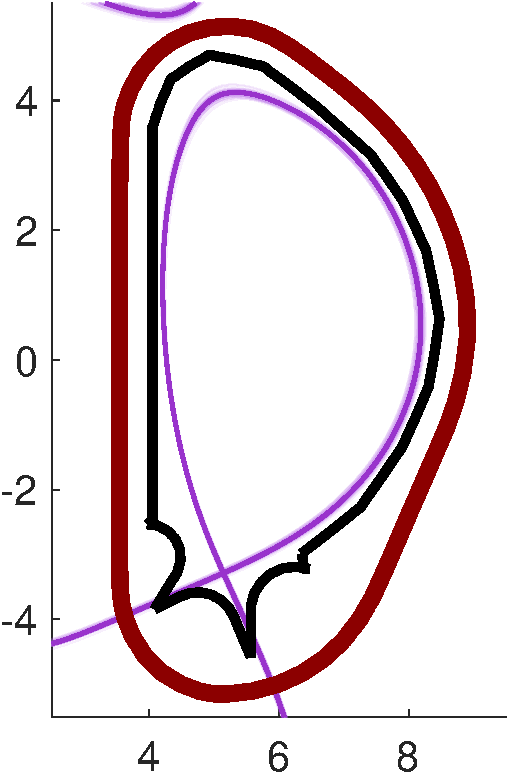
\includegraphics[width=0.19\linewidth]{./figures/QoI_MC_surrogate.pdf}
&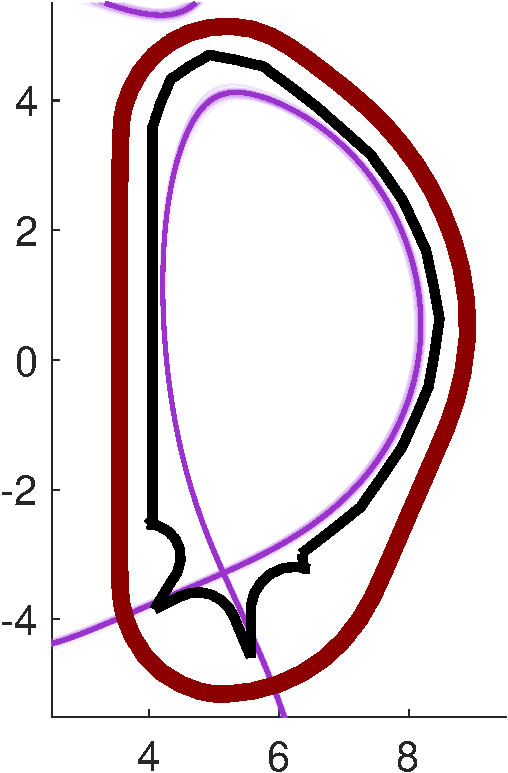
\includegraphics[width=0.19\linewidth]{./figures/QoI_MLMC_DirectSolver_Interp2CommonGrid.pdf} 
& 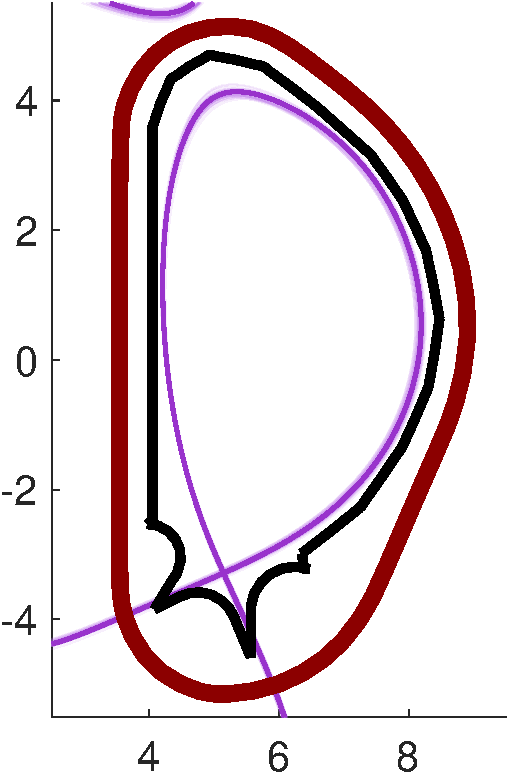
\includegraphics[width=0.19\linewidth]{./figures/QoI_MFMC.pdf} 
\\
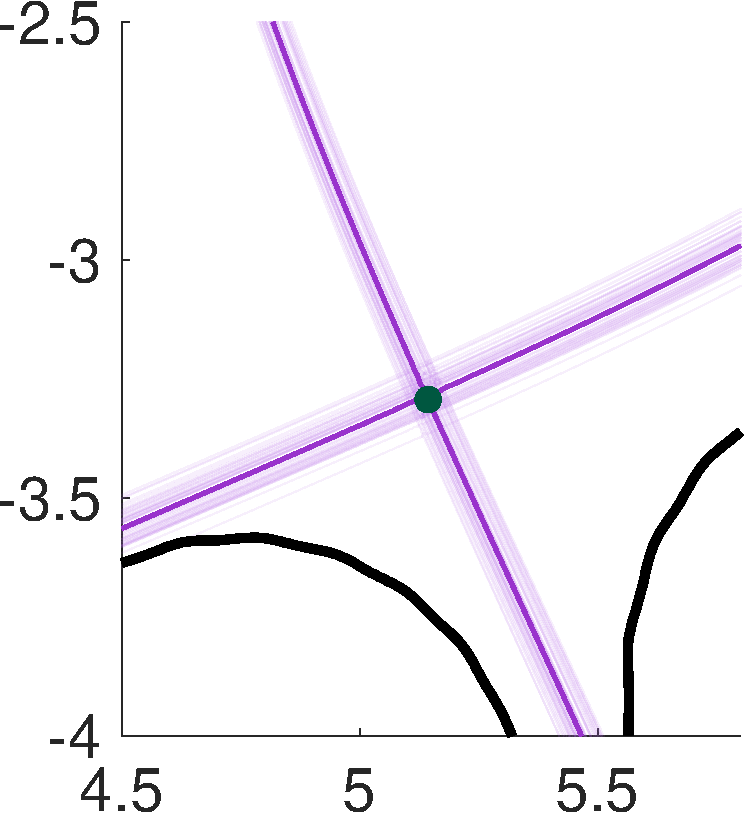
\includegraphics[width=0.19\linewidth]{./figures/QoI_MC_uniform_xptRegion.pdf} 
% &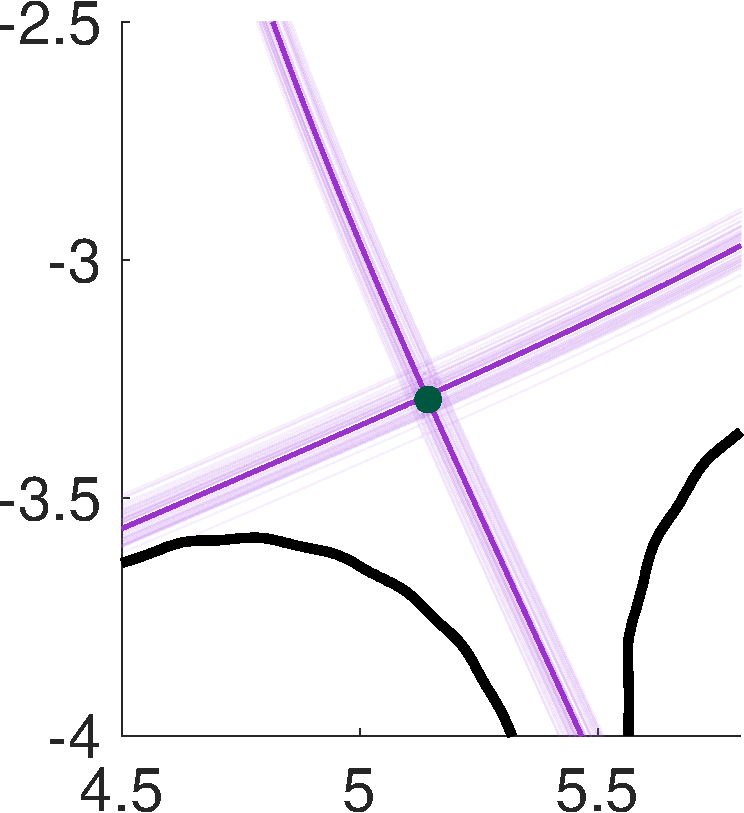
\includegraphics[width=0.19\linewidth]{./figures/QoI_MC_surrogate_xptRegion.pdf}
&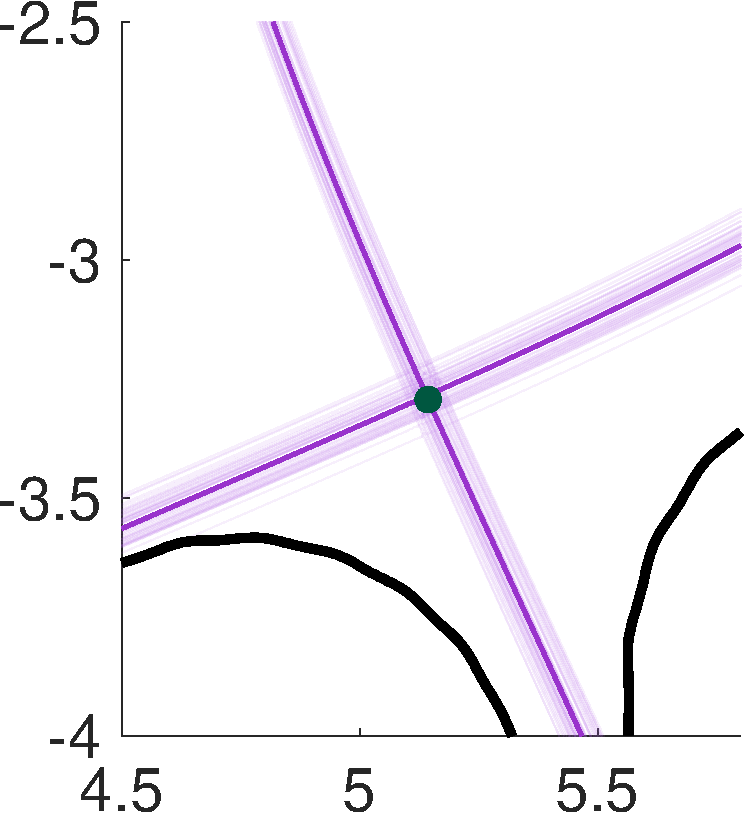
\includegraphics[width=0.19\linewidth]{./figures/QoI_MLMC_DirectSolver_xptRegion_Interp2CommonGrid.pdf} 
&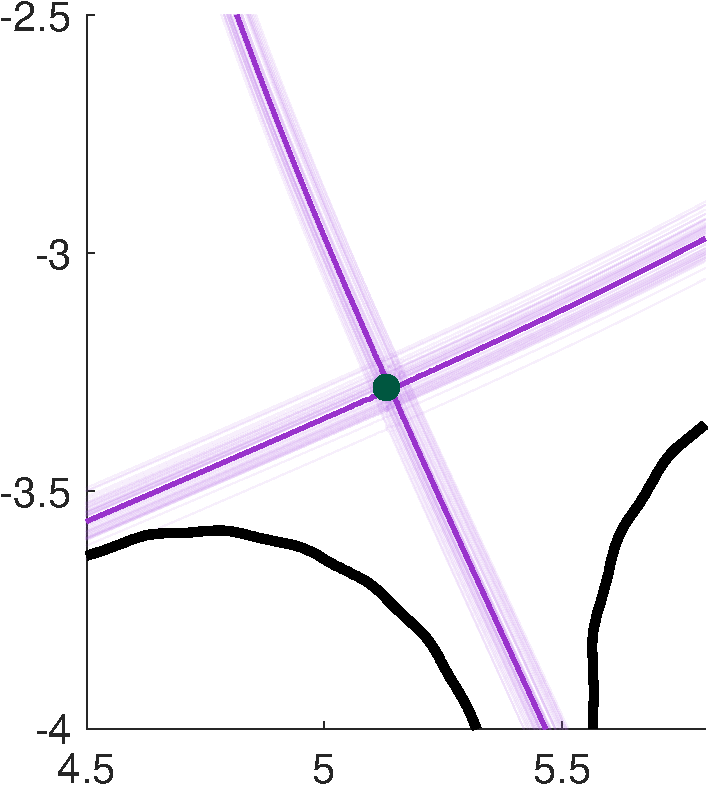
\includegraphics[width=0.19\linewidth]{./figures/QoI_MFMC_xptRegion.pdf} 
\\[1ex]
\quad MC-FE + Direct Solve &MLMC-FE + Direct Solve &MFMC-FE  \\[-0.5ex]
\end{tabular}
\caption{The overlayed plasma boundaries of 50 random realizations are 
displayed in the top row as violet curves (interpolated to the finest mesh with spatial grid level $\ell=4$). The solid violet line is the plasma boundary of the expected 
poloidal flux generated with tolerance $\epsilon=4\times 10^{-4}$. 
The inner and outer walls of the reactor are displayed in solid black and 
dark red respectively. The bottom row shows the regions close to the 
x-points in more detail. The dark green dots are the x-points of the expected 
solution. The columns from left to right correspond to simulations using the 
MC-FE approach with the direct solver and surrogate, MLMC-FE with direct 
solver and surrogate. All simulations were interpolated to the geometry-conforming uniform meshes of discretization level $\ell=4$.} 
\label{fig:QoI_plot}
\end{figure}
%





The sample size estimation for various $\epsilon$ is shown in Table \ref{Tab:SampleSize}.


%
\begin{table}[ht]
	\centering
			\scalebox{0.62}{
   \begin{tabular}{c|c|c|c|c|c|c|c|c|c|c|c|c|}
	    \cline{2-7}	
		&\multicolumn{6}{|c|}{ Level $\ell$}\\
			\hline
			\multicolumn{1}{|c|}{$\epsilon$}&0&1&2&3&4&5\\
			\hline
			\multicolumn{1}{|c|}{$8\times 10^{-3} $}&&&5&&&\\
			\multicolumn{1}{|c|}{$6\times 10^{-3} $}&&&9&&&\\
			\multicolumn{1}{|c|}{$4\times 10^{-3} $}&&&&21&&\\
			\multicolumn{1}{|c|}{$2\times 10^{-3} $}&&&&73&&\\
			\multicolumn{1}{|c|}{$10^{-3} $}&&&&&287&\\
			\multicolumn{1}{|c|}{$8\times 10^{-4} $}&&&&&445&\\
			\multicolumn{1}{|c|}{$6\times 10^{-4} $}&&&&&845&\\
                \multicolumn{1}{|c|}{$4\times 10^{-4} $}&&&&&2000&\\
                \multicolumn{1}{|c|}{$2\times 10^{-4} $}&&&&&& 8000$^{\ast}$\!\!\\
			\hline
	\end{tabular}
 \qquad
		\begin{tabular}{c|c|c|c|c|c|c|c|c|c|c|c|c|}
	    \cline{2-7}	
		&\multicolumn{6}{|c|}{ Level $\ell$}\\
			\hline
			\multicolumn{1}{|c|}{$\epsilon$}&0&1&2&3&4&5\\
			\hline
			\multicolumn{1}{|c|}{$8\times 10^{-3} $}&10     &2     &2&&&\\
			\multicolumn{1}{|c|}{$6\times 10^{-3} $}&12     &2     &2&&&\\
			\multicolumn{1}{|c|}{$4\times 10^{-3} $}&22     &5     &2     &2&&\\
			\multicolumn{1}{|c|}{$2\times 10^{-3} $}&163    &26     &5     &2&&\\
			\multicolumn{1}{|c|}{$10^{-3} $}&577   &90    &15     &3     &2&\\
			\multicolumn{1}{|c|}{$8\times 10^{-4} $}&1036 &157 &26 &5 &2&\\
			\multicolumn{1}{|c|}{$6\times 10^{-4} $}&1744 &266 &44 &9 &2&\\
                \multicolumn{1}{|c|}{$4\times 10^{-4} $}&3911 &553 &86 &17 &4&\\
                \multicolumn{1}{|c|}{$2\times 10^{-4} $}&15619 &2298 &370 &57 &12 &2\\
			\hline
	\end{tabular}
 \qquad
		\begin{tabular}{c|c|c|c|c|c|c|c|c|c|c|c|c|c|c|c|c|c|}
	    \cline{2-7}	
		&\multicolumn{6}{|c|}{ Level $\ell$}\\
			\hline
			\multicolumn{1}{|c|}{$\epsilon$}&0&1&2&3&4&5\\
			\hline
			\multicolumn{1}{|c|}{$8\times 10^{-3} $}&2&2&2&&&\\
			\multicolumn{1}{|c|}{$6\times 10^{-3} $}&2&2&2&&&\\
			\multicolumn{1}{|c|}{$4\times 10^{-3} $}&2&2&2&2&&\\
			\multicolumn{1}{|c|}{$2\times 10^{-3} $}&2&2&2&2&&\\
			\multicolumn{1}{|c|}{$10^{-3} $}&2&2&2&2&2&\\
			\multicolumn{1}{|c|}{$8\times 10^{-4} $}&2&2&2&2&2&\\
                \multicolumn{1}{|c|}{$6\times 10^{-4} $}&2&2&2&2&2&\\
			\multicolumn{1}{|c|}{$4\times 10^{-4} $}&2&2&2&2&2&\\
                \multicolumn{1}{|c|}{$2\times 10^{-4} $}&12&2&2&2&-&2\\
			\hline
	\end{tabular}
 
 }
	\caption{The optimal sample size estimation for MC-FE (left), uniform MLMC-FE (middle), and MFMC-FE (right). The simulations were conducted for a variety of choices of $\epsilon$. The computational cost associated with a tolerance of $\epsilon = 2\times 10^{-4}$ for Monte Carlo was prohibitive; the entry in the table for this tolerance (with an asterisk) is an estimate.}
	\label{Tab:SampleSize}
\end{table}
%

%
\begin{table}[ht]
	\centering
			\scalebox{0.62}{
   \begin{tabular}{c|c|c|c|c|c|c|c|c|c|c|c|c|}
			\hline
			\multicolumn{1}{|c|}{ }&MC-FE &MLMC-FE&MFMC-FE &MFMC-FE(Interp)\\
			\multicolumn{1}{|c|}{$\epsilon$}&Time & \begin{tabular}{cc} \,\,\,\,\,Time & \,\,\,Speedup \end{tabular} &\begin{tabular}{cc} \,\,\,\,Time & \,\,\,Speedup \end{tabular} &\begin{tabular}{cc} \,\,\,\,Time & \,\,\,Speedup \end{tabular}\\
			\hline
			\multicolumn{1}{|c|}{$8\times 10^{-3} $}&1.42e+01&\begin{tabular}{cc}6.61e+00\,\,\, & 2.1 \end{tabular}&\begin{tabular}{cc}7.3426e+00\,\,  &1.9339e+00 \end{tabular} &\begin{tabular}{cc}1.5563e+01\,\,  &9.1242e-01 \end{tabular} \\
			\multicolumn{1}{|c|}{$6\times 10^{-3} $}&2.75e+01&\begin{tabular}{cc}7.44e+00\,\,\, & 3.7 \end{tabular}&\begin{tabular}{cc}7.2427e+00\,\, &3.7969e+00 \end{tabular}&\begin{tabular}{cc}1.5389e+01&1.7870e+00
            \end{tabular}\\
			\multicolumn{1}{|c|}{$4\times 10^{-3} $}&6.60e+01&\begin{tabular}{cc}4.36e+01\,\,\, & 1.5 \end{tabular}&\begin{tabular}{cc}1.4342e+01&4.6019e+00\end{tabular}&\begin{tabular}{cc}2.5341e+01&2.6045e+00
            \end{tabular}\\
			\multicolumn{1}{|c|}{$2\times 10^{-3} $}&2.19e+02&\begin{tabular}{cc}4.73e+01\,\, & 4.6\end{tabular}&\begin{tabular}{cc}1.4278e+01&1.5338e+01 \end{tabular}&\begin{tabular}{cc}2.5618e+01&8.5487e+00
            \end{tabular}\\
			\multicolumn{1}{|c|}{$10^{-3} $}&4.66e+03&\begin{tabular}{cr}1.66e+02\,\, & 28.1 \end{tabular}&\begin{tabular}{cc}3.6678e+01&1.2705e+02\end{tabular}&\begin{tabular}{cc}4.9038e+01&9.5028e+01
            \end{tabular}\\
			\multicolumn{1}{|c|}{$8\times 10^{-4} $}&8.02e+03&\begin{tabular}{cc}4.33e+02\,\, & 18.5 \end{tabular}&\begin{tabular}{cc}4.2890e+01&1.8699e+02
            \end{tabular}&\begin{tabular}{cc}5.6344e+01&1.4234e+02
            \end{tabular}\\
			\multicolumn{1}{|c|}{$6\times 10^{-4} $}&1.49e+04&\begin{tabular}{cc}5.36e+02\,\, & 27.8 \end{tabular}&\begin{tabular}{cc}4.8741e+01 &3.0570e+02\end{tabular}&\begin{tabular}{cc}6.4086e+01&2.3250e+02
            \end{tabular}\\
                \multicolumn{1}{|c|}{$4\times 10^{-4} $}&3.66e+04&\begin{tabular}{cc}1.03e+03\,\, & 35.4 \end{tabular} &\begin{tabular}{cc}4.3724e+01&8.3707e+02 \end{tabular}&\begin{tabular}{cc}5.7562e+01&6.3584e+02
            \end{tabular}\\
                \multicolumn{1}{|c|}{$2\times 10^{-4} $}&5.84e+05$^{\ast}$\!\!\!&\begin{tabular}{cc}4.90e+03 &119.2 \end{tabular} &\begin{tabular}{cc}2.2876e+02&2.5529e+03 \end{tabular}&\begin{tabular}{cc}2.4207e+02 &2.4125e+03
            \end{tabular}\\
			\hline
	\end{tabular}
 }
	\caption{The CPU time in seconds for MC-FE (left), uniform MLMC-FE (middle), and MFMC-FE (right), together with speedups for the multilevel methods, for a variety of choices of $\epsilon$. The computational cost associated with a tolerance of $\epsilon = 2\times 10^{-4}$ for Monte Carlo was prohibitive; the entry in the table for this tolerance (with an asterisk) is an estimate.}
	\label{Tab:CPU_time}
\end{table}
%




\noindent \textbf{Geometric descriptors.}
%
\begin{table}[ht]
	\centering
			\scalebox{0.6}{
		\begin{tabular}{c|c|c|c|c|c|c|}
			\cline{2-5}
				&\multicolumn{1}{c|}{MC-FE DS}&MLMC-FE DS&MLMC-FE DS (Interp)&MLMC-FE Surrogate (Interp)\\
			\hline
			\multicolumn{1}{|c|}{x point}&(5.14,-3.29)&(5.14,-3.29)&(5.14,-3.29)&(5.14,-3.29)\\
			\hline
			\multicolumn{1}{|c|}{magnetic axis}&(6.41,0.61)&(6.44,0.56)&(6.41,0.61)&(6.41,0.61)\\
			\hline
			\multicolumn{1}{|c|}{strike} &(4.16,-3.71)&(4.16,-3.71)&(4.16,-3.71)&(4.16,-3.71)\\
			\multicolumn{1}{|c|}{points}&(5.56,-4.22)&(5.56,-4.22)&(5.56,-4.22)&(5.56,-4.22)\\
			\hline
			\multicolumn{1}{|c|}{inverse aspect ratio} &0.32&0.32&0.32&0.32\\
			\hline
			\multicolumn{1}{|c|}{elongation} &1.86&1.87&1.86&1.86\\
			\hline
			\multicolumn{1}{|c|}{upper triangularity}&0.43&0.43&0.43&0.43\\
			\hline
			\multicolumn{1}{|c|}{lower triangularity} &0.53&0.53&0.53&0.53\\
			\hline
	\end{tabular}
  }
	\caption{Geometric parameters of the expected poloidal flux $u$ from MC-FE with direct solver, MLMC-FE with direct solver,  MLMC-FE with direct solver with interpolating solution to a common fine grid of level $L=5$, MLMC-FE with surrogate with interpolating solution to a common fine grid of level $L=5$. The results are generated with an nMSE $4\times 10^{-4}$ on the geometry-conforming uniform mesh set.}
	\label{Tab: QoI_GeoInfo}
\end{table}






% % =============================
% \subsection{Uncertainties in the source term}
% % =============================
% In this experiment, we study the uncertainty in perturbing the reference parameter that characterizes the source term \eqref{eq:source}.
% \begin{table}[ht]
% 	\centering
% 			\scalebox{0.62}{
%    \begin{tabular}{c|c|c|c|c|c|c|c|c|c|c|c|c|}
% 	    \cline{2-7}	
% 		&\multicolumn{6}{|c|}{ Level $\ell$}\\
% 			\hline
% 			\multicolumn{1}{|c|}{$\epsilon$}&0&1&2&3&4&5\\
% 			\hline
% 			\multicolumn{1}{|c|}{$8\times 10^{-3} $}&&&8&&&\\
% 			\multicolumn{1}{|c|}{$6\times 10^{-3} $}&&&10&&&\\
% 			\multicolumn{1}{|c|}{$4\times 10^{-3} $}&&&&25&&\\
% 			\multicolumn{1}{|c|}{$2\times 10^{-3} $}&&&&93&&\\
% 			\multicolumn{1}{|c|}{$10^{-3} $}&&&&&423&\\
% 			\multicolumn{1}{|c|}{$8\times 10^{-4} $}&&&&&678&\\
% 			\multicolumn{1}{|c|}{$6\times 10^{-4} $}&&&&&1211&\\
%                 \multicolumn{1}{|c|}{$4\times 10^{-4} $}&&&&&2700$^{\ast}$&\\
%                 \multicolumn{1}{|c|}{$2\times 10^{-4} $}&&&&&&11000$^{\ast}$\!\!\\
% 			\hline
% 	\end{tabular}
%  \qquad
% 		\begin{tabular}{c|c|c|c|c|c|c|c|c|c|c|c|c|}
% 	    \cline{2-7}	
% 		&\multicolumn{6}{|c|}{ Level $\ell$}\\
% 			\hline
% 			\multicolumn{1}{|c|}{$\epsilon$}&0&1&2&3&4&5\\
% 			\hline
% 			\multicolumn{1}{|c|}{$8\times 10^{-3} $}&10 &2 &2&&&\\
% 			\multicolumn{1}{|c|}{$6\times 10^{-3} $}&11 &3 &2 &&&\\
% 			\multicolumn{1}{|c|}{$4\times 10^{-3} $}&33 &7 &2 &2&&\\
% 			\multicolumn{1}{|c|}{$2\times 10^{-3} $}&150 &27 &4 &2&&\\
% 			\multicolumn{1}{|c|}{$10^{-3} $}&692 &116 &19 &4 &2&\\
% 			\multicolumn{1}{|c|}{$8\times 10^{-4} $}&1008 &160 &27 &6 &2&\\
% 			\multicolumn{1}{|c|}{$6\times 10^{-4} $}&2022 &322 &53 &10 &3&\\
%                 \multicolumn{1}{|c|}{$4\times 10^{-4} $}&4158 &613 &106 &14 &4&\\
%                 \multicolumn{1}{|c|}{$2\times 10^{-4} $}&17158 &2612 &442 &59 &13 &2\\
% 			\hline
% 	\end{tabular}
%  \qquad
% 		\begin{tabular}{c|c|c|c|c|c|c|c|c|c|c|c|c|c|c|c|c|c|}
% 	    \cline{2-7}	
% 		&\multicolumn{6}{|c|}{ Level $\ell$}\\
% 			\hline
% 			\multicolumn{1}{|c|}{$\epsilon$}&0&1&2&3&4&5\\
% 			\hline
% 			\multicolumn{1}{|c|}{$8\times 10^{-3} $}&&&&&&\\
% 			\multicolumn{1}{|c|}{$6\times 10^{-3} $}&&&&&&\\
% 			\multicolumn{1}{|c|}{$4\times 10^{-3} $}&&&\\
% 			\multicolumn{1}{|c|}{$2\times 10^{-3} $}&&&\\
% 			\multicolumn{1}{|c|}{$10^{-3} $}&&&&&&\\
% 			\multicolumn{1}{|c|}{$8\times 10^{-4} $}&&&&&&\\
%                 \multicolumn{1}{|c|}{$6\times 10^{-4} $}&&&&&&\\
% 			\multicolumn{1}{|c|}{$4\times 10^{-4} $}&&&&&&\\
%                 \multicolumn{1}{|c|}{$2\times 10^{-4} $}&&&&&&\\
% 			\hline
% 	\end{tabular}
 
%  }
% 	\caption{The optimal sample size estimation for MC-FE (left), uniform MLMC-FE (middle), and MFMC-FE (right). The simulations were conducted for a variety of choices of $\epsilon$. The computational cost associated with a tolerance of $\epsilon = 2\times 10^{-4}$ for Monte Carlo was prohibitive; the entry in the table for this tolerance (with an asterisk) is an estimate.}
% 	\label{Tab:SampleSize_Source_Term}
% \end{table}

% \begin{table}[ht]
% 	\centering
% 			\scalebox{0.62}{
%    \begin{tabular}{c|c|c|c|c|c|c|c|c|c|c|c|c|}
% 			\hline
% 			\multicolumn{1}{|c|}{ }&MC-FE &MLMC-FE &MFMC-FE\\
% 			\multicolumn{1}{|c|}{$\epsilon$}&Time & \begin{tabular}{cc} \,\,\,\,\,Time & \,\,\,Speedup \end{tabular}  &\begin{tabular}{cc} \,\,\,\,Time & \,\,\,Speedup \end{tabular}\\
% 			\hline
% 			\multicolumn{1}{|c|}{$8\times 10^{-3} $}&9.71e+01&\begin{tabular}{cc}1.10e+01\,\,\, & 8.8 \end{tabular}&\begin{tabular}{cc}..\,\,  & .. \end{tabular} \\
% 			\multicolumn{1}{|c|}{$6\times 10^{-3} $}&1.16e+02&\begin{tabular}{cc}1.27e+01\,\,\, & 9.1 \end{tabular}&\begin{tabular}{cc}..\,\, &.. \end{tabular}\\
% 			\multicolumn{1}{|c|}{$4\times 10^{-3} $}&1.29e+02&\begin{tabular}{cc}3.39e+01\,\,\, & 3.8 \end{tabular}&\begin{tabular}{cc}..& .. \end{tabular}\\
% 			\multicolumn{1}{|c|}{$2\times 10^{-3} $}&8.03e+02&\begin{tabular}{cc}7.29e+01\,\, & 11.0\end{tabular}&\begin{tabular}{cc}..& .. \end{tabular}\\
% 			\multicolumn{1}{|c|}{$10^{-3} $}&1.49e+04&\begin{tabular}{cr}2.55e+02\,\, & 58.5 \end{tabular}&\begin{tabular}{cc}..& .. \end{tabular}\\
% 			\multicolumn{1}{|c|}{$8\times 10^{-4} $}&3.89e+04&\begin{tabular}{cc}2.76e+02\,\, &140.6 \end{tabular}&\begin{tabular}{cc}..& ..
%             \end{tabular}\\
% 			\multicolumn{1}{|c|}{$6\times 10^{-4} $}&1.1219e+05&\begin{tabular}{cc}7.1946e+02\,\, & .. \end{tabular}&\begin{tabular}{cc}.. & .. \end{tabular}\\
%                 \multicolumn{1}{|c|}{$4\times 10^{-4} $}&..&\begin{tabular}{cc}1.1598e+03\,\, & .. \end{tabular} &\begin{tabular}{cc}..& .. \end{tabular}\\
%                 \multicolumn{1}{|c|}{$2\times 10^{-4} $}&..$^{\ast}$\!\!\!&\begin{tabular}{cc}4.4956e+03 &.. \end{tabular} &\begin{tabular}{cc}..&.. \end{tabular}\\
% 			\hline
% 	\end{tabular}
%  }
% 	\caption{The CPU time in seconds for MC-FE (left), uniform MLMC-FE (middle), and MFMC-FE (right), together with speedups for the multilevel methods, for a variety of choices of $\epsilon$. The computational cost associated with a tolerance of $\epsilon = 2\times 10^{-4}$ for Monte Carlo was prohibitive; the entry in the table for this tolerance (with an asterisk) is an estimate.}
% 	\label{Tab:CPU_time_Source_Term}
% \end{table}